\documentclass[border=10pt,tikz,crop]{standalone}
\usetikzlibrary{decorations.pathmorphing}
\thispagestyle{empty}
\usetikzlibrary{shapes.geometric}
\begin{document}
	
	

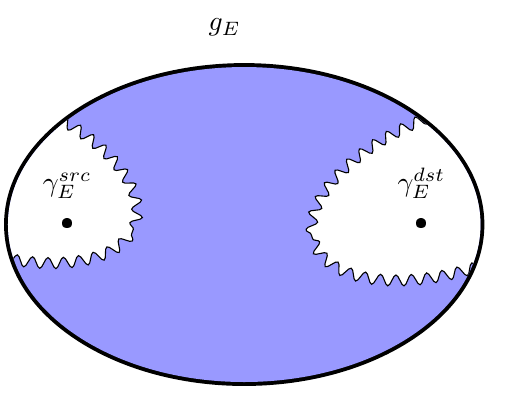
\begin{tikzpicture}
%\draw[help lines] (0,0) grid (10,10);


\draw[fill=blue!60] (1.75,1) ellipse (3cm and 2cm);
\node at (1.5,3.5) {\textbf{$g_E$}};

\begin{scope}   
	\pgfset{minimum width=6cm,minimum height=4cm}
	\pgfsetlinewidth{1mm}
	\pgftransformshift{\pgfpoint{1.75cm}{1cm}}
	\pgfnode{ellipse}{center}{}{nodename}{\pgfusepath{stroke,clip}}
	%Cleaning up the mess we caused
	\pgftransformreset
	\pgfsetlinewidth{0.4pt} 
	\pgfset{minimum width=1pt,minimum height=1pt}
	% Back to drawing
	\fill[blue!40] (-2cm,-2cm) rectangle (5cm,4cm);

\draw[rotate around={-20:(0,0)},decoration={snake, amplitude=.7mm, segment length=2mm}, decorate,fill=white] (-2,1) ellipse (2cm and 1cm);
\draw[rotate around={200:(4.5,1.5)},decoration={snake, amplitude=.7mm, segment length=2mm}, decorate,fill=white] (4.5,1.5) ellipse (2cm and 1cm);


\end{scope}

\node[label=above:{$\gamma_E^{dst}$}] at (4,1) (dst) {\textbullet};
\node[label=above:{$\gamma_E^{src}$}] at (-.5,1) (src) {\textbullet};

\pgfresetboundingbox
\path[use as bounding box] (-1,-1) rectangle (4.8,3.5);
\end{tikzpicture}
\end{document}